%===================================================================================
% Chapter: Extracción de Información
%===================================================================================
\chapter{Extracción de Información}\label{chapter:information_extraction}
\addcontentsline{toc}{chapter}{Extracción de Información}

\section{Extracción de Entidades}

Una entidad nombrada es una palabra o frase que identifica un objeto de un conjunto de objetos que tienen atributos similares. Ejemplos de esto son las personas, las organizaciones, drogas, nombres de enfermedades dentro del dominio m\'edico, entre otros. \textbf{Reconocimiento de Entidades Nombradas} (\textbf{NER}) es el proceso de localizar y clasificar entidades nombradas en un texto dentro de un conjunto de categor\'ias predefinidas de entidades.
Formalmente, dada una secuencia de \emph{tokens} $s=<w_1, w_2, ..., w_N >$, NER devuelve como salida una lista de tuplas $<I_s, I_e, t>$, una por cada entidad mencionada en s, donde $I_s \in [1,...,N]$ y $I_e \in [1,...,N]$ son el inicio y el fin de los \'indices de la entidad nombrada mencionada; y $t$ es el tipo de la misma dentro de una categor\'ia predefinida~\cite{li2018survey}. 

NER es un paso importante de preprocesamiento para una variedad de problemas tales como Recuperaci\'on de Informaci\'on, Preguntas y Respuestas, Traducci\'on de m\'aquina, etc.


\subsection{Enfoque Basado en Reglas}

Los sistemas de NER basados en reglas dependen de \emph{hand-crafted rules}. Las reglas pueden ser dise\~nadas basadas en el dominio espec\'ifico \emph{gazetteers}~\cite{etzioni2005unsupervised} y en patrones sint\'acticos-l\'exicos~\cite{zhang2013unsupervised}. En el dominio biom\'edico~\cite{hanisch2005prominer} se propuso \emph{ProMiner} el cual utiliza un diccionario de sin\'onimos preprocesado para identificar prote\'inas en texto biom\'edico.

Otros sistema de NER basado en reglas conocido es \textbf{NetOwl}~\cite{krupka2005description}. Este tipo de sistemas consisten esencialmente en \emph{hand-crafted semantic} y reglas sint\'acticas para reconocer entidades. Los sistemas basados en reglas trabajan bien cuando el lexicon es exhaustivo, a su vez con las reglas de dominio espec\'ifico y diccionarios incompletos, alta precisi\'on y bajo recobrado son comunmente observados en estos sistemas. Adem\'as estos sistemas no pueden ser trasnferidos a otros dominios~\cite{li2018survey}.


\subsection{Enfoques de Aprendizaje no Supervisado}  

Uno de los t\'ipicos enfoques de aprendizaje no supervisado es \emph{clustering}~\cite{nadeau2007survey}. Los sistemas de NER basados en \emph{clustering} extraen entidades nombradas de los distintos \emph{clusters} basado en las similiridades del contexto. La idea esencial es que recursos l\'exicos, patrones l\'exicos y estad\'isticas computadas en grandes corpus pueden ser utilizadas para inferir entidades nombradas~\cite{li2018survey}.

Un sistema no supervisado para la construcci\'on de \emph{gazetteers} y la resoluci\'on de la ambiguedad entre entidades nombradas fue presentado por~\cite{nadeau2006unsupervised}. Este sistema combina NER y la 
desambiguación de las entidades, basado en simples heur\'isticas. Enfoques no supervisados para NER en textos biom\'edicos ha sido presentado por~\cite{zhang2013unsupervised}, donde su modelo depende de terminolog\'ias, estad\'isticas en corpus~(la frecuencia de documentos inversa y vectores de contexto) y \emph{shallow syntactic knowledge} (e.g, \emph{noun phrase chunking}). Los experimentos en dos conjuntos de datos biom\'edicos demuestran la efectividad y capacidad de generalizaci\'on de su enfoque no supervisado.


\subsection{Enfoque de Aprendizaje Supervisado Basado en Rasgos}

Cuando se aplica aprendizaje supervisado, el problema de NER consiste en una tarea de multiclasificaci\'on o etiquetado de secuencias. Donde dados, ejemplos anotados y rasgos dise\~nados para representar cada ejemplo entrenante, los algoritmos de aprendizaje de m\'aquinas son utilizados para aprender el modelo para reconocer patrones similares de datos no vistos~\cite{li2018survey}.

El dise\~no de rasgos es esencial en los sistemas supervisados de NER. La representaci\'on por un vector de rasgos es una abstracci\'on sobre el texto donde una palabra es representada por uno o muchos valores booleanos, num\'ericos o nominales~\cite{sekine2009named}. Existen rasgos a nivel de palabras (e.g \emph{case}, morfolog\'ia y \emph{part-of-speech tag}~\cite{settles2004biomedical},~\cite{liao2009simple}), lista de \emph{lookup features}(e.g. \emph{Wikipedia} gazetteer y \emph{DBpedia} gazetteer~\cite{hoffart2011robust}) y rasgos de documentos y corpus (e.g. sintaxis local y m\'ultiples ocurrencias~\cite{ji2016joint}).

Utilizando estos rasgos muchos algoritmos de aprendizaje de m\'aquina supervisados han sido aplicados en \textbf{NER}. Ejemplo de esto son \emph{Hidden Markov Models} (\textbf{HMM})~\cite{bikel1999algorithm}, \emph{Decision Trees}~\cite{szarvas2006multilingual}, \emph{Maximum Entropy Models}~\cite{bender2003maximum}, \emph{Support Vector Machines}(\textbf{SVM})~\cite{li2004svm} y \emph{Conditional Random Fields}(\textbf{CRF})~\cite{settles2004biomedical},~\cite{lafferty2001conditional}.

\subsection{Enfoque Basado en T\'ecnicas de Aprendizaje Profundo}
En los \'ultimos a\~nos modelos para NER basados en aprendizaje profundo se han vuelto dominante. En comparaci\'on con enfoques basados en rasgos, el aprendizaje profundo es capaz de descubrir rasgos ocultos autom\'aticamente~\cite{li2018survey}. La figura~\ref{fig:NerDeepBased} muestra la arquitectura general de un modelo de aprendizaje profundo enfocado a resolver el problema de NER. 

Existen 3 ventajas esenciales de aplicar t\'ecnicas de aprendizaje profundo para resolver NER. En primer lugar, NER se beneficia de la aplicaci\'on de transformaciones no lineares, lo cual genera mapeos no lineares de la entrada hacia la salida, a diferencia de modelos lineares como HMM. En segundo lugar, el aprendizaje profundo ahorra esfuerzo significativo para dise\~nar NER \emph{features}. Y en tercer lugar, los modelos de aprendizaje profundo para NER pueden ser entrenados con un paradigma \emph{end-to-end}, usando descenso por gradiente~\cite{li2018survey}.

\begin{figure}[h!]
	\centering
	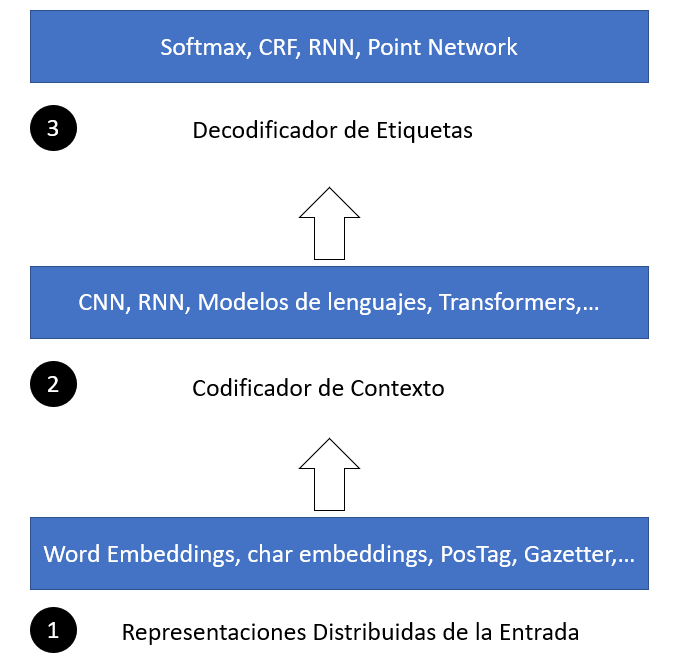
\includegraphics[width = 10cm]{Imagenes/NERDeep.png}
	\caption{Arquitectura general de aprendizaje profundo para NER.}\label{fig:NerDeepBased}
\end{figure}

\subsection{Representaci\'on Distribuida de la Entrada}

%Una primera opci\'on para la representaci\'on de una palabra es el \emph{one-hot vector}. En el espacio de los \emph{one-hot vector}, dos palabras tienen completamente dos diferentes representaciones y son ortogonales. Las representaciones distribuidas representan palabras en vectores densos de valores reales con peque\~na dimensi\'on donde cada dimensi\'on representa un rasgo latente. Las representaciones distribuidas capturan propiedades sem\'anticas y sint\'acticas de la palabra.    

Algunos estudios~\cite{strubell2017fast} utilizan representaciones a nivel de palabras que son tipicamente pre-entrenadas sobre un largo n\'umero de colecciones de texto a trav\'es de algoritmos no supervisados tales como \emph{continuous bag of words (CBOW)} y \emph{continuous skip-gram models}~\cite{mikolov2013efficient}. En la figura~\ref{fig:cbowSkip} se muestra como \emph{CBOW} predice la palabra actual basada en el contexto y \emph{Skip-gram} predice las palabras del contexto dada la palabra actual. Estudios recientes como~\cite{yang2018design} han mostrado la importancia de los \emph{word embeddings} pre-entrenados. Entre los m\'as comunes se encuentran \emph{Word2Vec}~\footnote{https://code.google.com/archive/p/word2vec/} y \emph{GloVe}~\footnote{http://nlp.stanford.edu/projects/glove/}. En el caso de NER en el dominio biom\'edico se encuentra \emph{Bio-NER}~\cite{yao2015biomedical}, donde la represenatci\'on de palabras del mismo es entrenado en la base de datos de \emph{PubMed} usando un modelo \emph{skip-gram}. Otros trabajos que utilizan  representaciones a nivel de palabra son~\cite{ma2016end} y~\cite{wang2018code}.

\begin{figure}[h!]
	\centering
	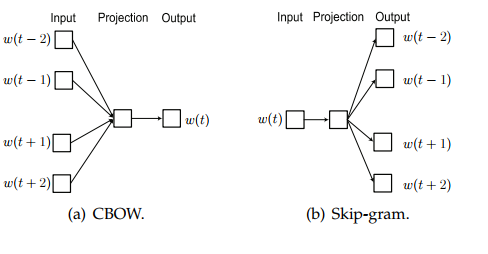
\includegraphics[width = 10cm]{Imagenes/CBOW_SkipGram.png}
	\caption{Arquitectura de CBOW y Skip-gram.}\label{fig:cbowSkip}
\end{figure}


Otra de las representaciones utilizadas en estudios como~\cite{li2018segbot} son las basadas en los caracteres de las palabras, la cual se aprende a partir de un modelo de redes neuronales \emph{end-to-end}~\cite{li2018survey}. La representaci\'on a nivel de caracteres ha mostrado ser \'util para explotar informaci\'on por debajo del nivel de la palabra tales como prefijo y sufijos. Adem\'as posee la ventaja de otorgar una representaci\'on a las palabras que incluso no pertenezcan al vocabulario y compartir informaci\'on a nivel de regularidades y morfemas. Las dos arquitecturas m\'as utilizadas para extraer representaci\'on a nivel de caracteres son las basadas en modelos de \emph{Convolutional Neural Networks} (\textbf{CNN})~\cite{ma2016end} y las basadas en modelos de \emph{Recurrent Neural Networks} (\textbf{RNN})~\cite{lample2016neural}. En trabajos como~\cite{gridach2017character} se utilizan ambas representaciones para reconocer entidades biomedicas. La figura~\ref{fig:charLevel} muestra los dos tipos de arquitecturas.

\begin{figure}[h!]
	\centering
	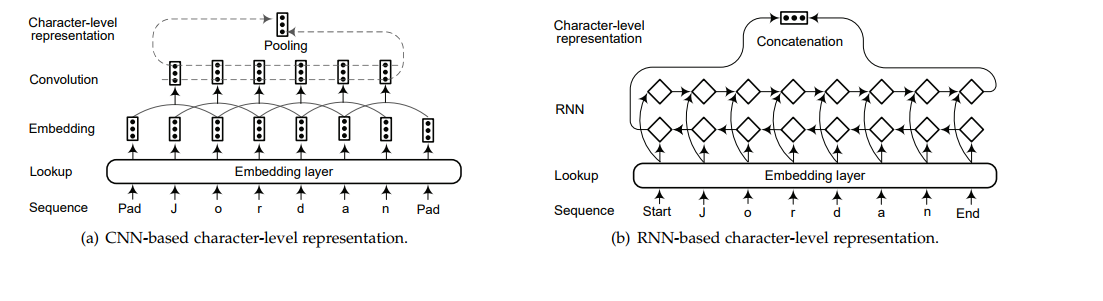
\includegraphics[width = 10cm]{Imagenes/charEmb.png}
	\caption{Modelos basados en CNN y RNN para la extracci\'on de la representaci\'on de la palabra a nivel de caracteres.}\label{fig:charLevel}
\end{figure}

Tambi\'en existen representaciones h\'ibridas donde adem\'as de representaciones a nivel de palabras y caracteres, incorporan informaci\'on adicional como los \emph{gazetteers}~\cite{huang2015bidirectional} y similaridad l\'exica~\cite{ghaddar2018robust}. A\~nadir informaci\'on extra puede mejorar el desempe\~no de NER pero a su vez puede da\~nar la generalizaci\'on de estos sistemas. Un ejemplo de esto es el modelo \emph{BiLSTM-CRF} presentado en~\cite{huang2015bidirectional} donde 4 tipos de rasgos fueron utilizados: \emph{spelling features}, \emph{context features}, \emph{word embeddings} y \emph{gazetteers}, los resultados muestran que el uso de rasgos extras como los \emph{gazetteers} incrementan la precisi\'on del sistema. El art\'iculo~\cite{wei2016disease} presenta un sistema de redes neuronales basado en CRF para el reconocimiento y normalizaci\'on de nombres de enfermedades; este sistema utiliza \emph{word embeddings} incluyendo, \emph{POS tags}, \emph{chunking} y rasgos correspondientes a la forma de las palabras (i.e, diccionarios y rasgos morfol\'ogicos). Actualmente uno de los modelos de representaci\'on de lenguajes m\'as utilizados es \emph{Bidirectional Encoder Representations from Transformers} (\textbf{BERT})~\cite{devlin2018bert} que utiliza modelos de lenguaje enmascarados para permitir el pre-entrenamiento de representaciones bidireccionales. Para un \emph{token} determinado, su representaci\'on es compuesta por su posici\'on correspondiente, segmento y \emph{token embeddings}.


\subsection{Redes Neuronales Convolucionales}
%Las CNN son un algoritmo de aprendizaje de m\'aquina, donde desde lo m\'as b\'asico pueden ser vistas como una especie de red neuronal que utiliza muchas copias del mismo neur\'on. Esto permite a la red tener muchos neurones y expresar computacionalmente enormes modelos mientras conserva el n\'umero actual de par\'ametros. Las CNN se utilizan fundamentalmente en el procesamiento de im\'agenes, pero forman parte tambi\'en del estado del arte del procesamiento de lenguaje natural actualmente.
%
%Su funcionamiento se basa fundamentalmente en la operaci\'on de convoluci\'on. La misma utiliza una ventana denominada \emph{kernel}. Un \emph{kernel} es una matriz pequeña cuyos valores son los par\'ametros de las capas convolucionales. La misma se desliza por el vector de entrada (una oraci\'on por ejemplo), efectuando una operaci\'on de producto escalar para producir la salida. La distancia entre cada salto del kernel se denomina \emph{stride}.(PONER PAPER DE EXPLICACION DE UNA CNN) 

Un ejemplo de un acercamiento a partir de CNN al problema de NER es el presentado en~\cite{collobert2011natural} donde una palabra es etiquetada teniendo en consideraci\'on la oraci\'on completa. Cada palabra en la secuencia de entrada se representa a partir de un vector $N-dimensional$ despu\'es de la fase de representaci\'on de la entrada. Luego, una CNN es usada para producir rasgos locales alrededor de cada palabra y el tama\~no de la salida de las capas convolucionales depende del n\'umero de palabras en la oraci\'on. El vector de rasgos global se construye combinando los vectores de rasgos locales extra\'idos por las capas convolucionales. La dimensi\'on del vector global de salida es fija en orden de aplicar \emph{subsequent affine layers}. Finalmente, este vector de rasgos global de dimensi\'on fija es la entrada del decodificador de etiquetas para computar la distribuci\'on de las puntuaciones para cada una de la etiquetas. Siguiendo el trabajo~\cite{collobert2011natural} se encuentra el sistema \emph{Bio-NER} para el reconocimiento de entidades en textos biom\'edicos~\cite{yao2015biomedical}. Tambi\'en se resaltan art\'iculos utilizando CNN para el problema de NER como~\cite{zhou2017joint}.

\subsection{Redes Neuronales Recurrentes}

%Las redes neuronales recurrente son un algoritmo de aprendizaje de m\'aquinas, donde las conexiones entre los nodos forman un grafo dirigido dentro de una secuencia temporal. A diferencia de las \emph{Feedforward Neural Networks}, las \textbf{RNN} pueden utilizar su estado interno (memoria) para procesar secuencias de entrada. Lo cual hace que se utilice esencialmente en tareas como segmentaci\'on, reconocimiento de escritura a mano, reconocimiento del habla, extracci\'on y clasificaci\'on de palabras claves y extracci\'on de relaciones entre palabras claves en una oraci\'on. La red neuronal recurrente incluye conexiones que apuntan "hacia atr\'as", una especie de retroalimentaci\'on entre las neuronas dentro de las capas, a diferencia de otras redes cuya funci\'on de activaci\'on solo act\'ua en una direcci\'on.(PONER REFERENCIA DE DONDE SE EXPLIQUEN LAS RNN).

%Las \textbf{RNN} junto sus variantes tales como \emph{Gated Recurrent Unit} (\textbf{GRU}) y \emph{Long Short Term Memory} (\textbf{LSTM}), han demostrado notables logros en la modelaci\'on de datos secuenciales. En particular, las \textbf{RNN} bidireccionales hacen uso eficientemente de informaci\'on pasada (v\'ia \emph{forward states}) e informaci\'on futura (v\'ia \emph{backward states}) para un espec\'ifico time frame~\cite{huang2015bidirectional}. Por lo tanto, un \emph{token} codificado por una \textbf{RNN} bidireccional va a contener informaci\'on de toda la oraci\'on. 

El trabajo de \emph{Huang et al.}\cite{huang2015bidirectional} est\'a entre los primeros en utilizar una arquitectura de BiLSTM-CRF para el etiquetado de secuencias. Siguiendo este trabajo muchos trabajos como~\cite{chiu2016named},~\cite{ma2016end},~\cite{wei2016disease} aplican BiLSTM como la arquitectura b\'asica para codificar la informaci\'on de contexto. \emph{Yang et al.}~\cite{yang2016multi} utiliz\'o profundas \emph{Gate Recurrent Units} (\textbf{GRU}) tanto a nivel de caracteres como de palabras para codificar la morfolog\'ia y la informaci\'on contextual. Trabajos recientes como~\cite{katiyar2018nested},~\cite{ju2018neural} dise\~naron una red neuronal basada en \emph{Long Short Term Memory} (\textbf{LSTM}) para el reconocimiento de entidades nombradas que se encuentran solapadas. Particularmente el trabajo~\cite{ju2018neural} propuso un modelo de redes neuronales para identificar entidades solapadas apilando \emph{flat NER layers} din\'amicamente hasta que ninguna entidad externa es extra\'ida. En la figura~\ref{fig:RNN} se aprecia una arquitectura para NER basada en RNN.

\begin{figure}[h!]
	\centering
	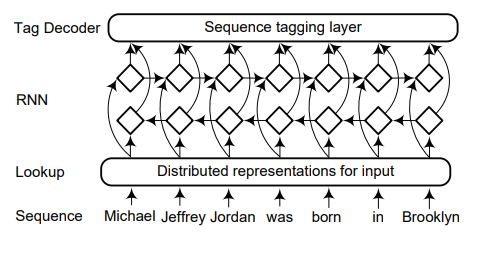
\includegraphics[width = 10cm]{Imagenes/RNN_Arquitecture.png}
	\caption{Modelo para \textbf{NER} basado en \textbf{RNN}.}\label{fig:RNN}
\end{figure}

%\subsection{Redes Neuronales Recursivas}
%
%Las redes neuronales recursivas son modelos adaptativos no lineales que son capaces de aprender informaci\'on estructurada profunda a partir de explorar una estructura dada en un orden topol\'ogico~\cite{li2018survey}. Las entidades nombradas est\'an altamente relacionadas a constituyentes lingu\'isticos como los sustantivos~\cite{li2017leveraging}. Sin embargo, un acercamiento t\'ipico para el etiquetado de secuencias toma en poca consideraci\'on la estructura de las frases de las oraciones. \emph{Li et al.}~\cite{li2017leveraging} propuso clasificar cada nodo en una estructura constituyente para \textbf{NER}. Este modelo calcula recursivamente los vectores ocultos de estado de cada nodo y los clasifica seg\'un los vectores ocultos.

\subsection{Neural Languaje Model}

%Los modelos de lenguajes es una familia de modelos describiendo la generaci\'on de secuencias. Dada una secuencia de \emph{tokens} $(t_1, t_2, ..., t_N)$, un \emph{forward language model} computa la probabilidad de la secuencia a partir de modelar la probabilidad del \emph{token} $t_k$ dado su historia $(t_1,...,t_{k-1})$~\cite{peters2017semi}.
%
%\begin{equation}
%	p(t_1, t_2, ..., t_N) = \prod_{k=1}^{N} p(t_k | t_1, t_2, ..., t_{k-1})
%\end{equation}
%
%
%A \emph{backward language} model es similar a un \emph{forward language} model, excepto que corre por la secuencia en orden reverso, prediciendo el \emph{token} dado el contexto futuro:
%
%\begin{equation}
%p(t_1, t_2, ..., t_N) = \prod_{k=1}^{N} p(t_k | t_{k + 1}, t_{k + 2}, ..., t_N)
%\end{equation}
%
%Para los modelos de lenguajes neuronales, la probabilidad del \emph{token} $t_k$ puede ser calculada a partir de la salida de una \textbf{RNN}. En cada posici\'on $k$, se puede obtener dos representaciones dependientes del contexto (forward and backward) y entonces combinarlas como el embedding de lenguaje del modelo final para el \emph{token} $t_k$.

Los modelos de lenguaje aumentado han sido emp\'iricamente verificados como \'util en numerosas tareas de etiquetado incluida NER~\cite{liu2018efficient},~\cite{liu2018empower} donde se utiliza una arquitectura conocida como \emph{LM-BiLSTM-CRF} (el \emph{LM} responde a \emph{Language Model}) donde el modelo de lenguaje y el modelo de etiquetado de secuencia comparten la misma capa a nivel de caracteres en una forma \emph{multi-task}. Los vectores de los \emph{embeddings} a nivel de caracteres, los \emph{word embeddings} pre-entrenados y la representaci\'on del modelo de lenguaje para cada palabra son concatenados y sirven de entrada para las LSTM a nivel de palabra. \emph{Peter et al.}~\cite{peters2018deep} propone la representaci\'on \emph{Embeddings from Language Models} (\textbf{ELMo}) que es computada encima de dos capas de modelos de lenguaje bidireccional con convoluciones de caracteres. Este nuevo tipo de representaci\'on contextualizada profunda de una palabra es capaz de modelar caracter\'isticas complejas del uso de la palabra (sem\'antica y sintaxis), as\'i como el uso de variaciones a trav\'es de distintos contextos lingu\'isticos (polysemy) y ha sido utilizada en tareas de \emph{NER} obteniendo buenos resultados como se muestra en el art\'iculo~\cite{jin2019probing}. La figura~\ref{fig:LM} muestra las diferencias entre las arquitecturas de los modelos pre-entrenados.

\subsection{Deep Transformer}

%Modelos neuronales para el etiquetado de secuencias est\'an t\'ipicamente basados en complejas \textbf{CNN} o \textbf{RNN} que consisten de un \emph{encoder} y un \emph{decoder}. Los \emph{Transformers} propuestos por~\cite{vaswani2017attention} son una arquitectura \emph{sequence-to-sequence}(\textbf{Seq2Seq}) que hacen uso de los mecanismos de atenci\'on, los cuales deciden en cada paso, que partes de la secuencia son relevantes a partir de las capas de \textbf{self-attention} o \textbf{multi-headed-attention}. 

Experimentos en varios tasks~\cite{kitaev2018constituency},~\cite{liu2018generating} muestran que los \emph{Transformers}~\cite{vaswani2017attention} son superiores en calidad y adem\'as requieren de significativamente menos tiempo para entrenar. Basado en \emph{Transformers} est\'a~\cite{radford2018improving} que propone \emph{Generative Pretrained Transformer} (\textbf{GPT}) para la tarea del entendimiento de lenguaje. A diferencia de GPT que es una arquitectura de izquierda a derecha, se encuentra BERT~\cite{devlin2018bert}. La representaci\'on pre-entrenada de BERT puede ser \emph{fine-tune} con una capa de salida adicional para un amplio rango de tareas, incluyendo NER. En la figura~\ref{fig:transformer} se aprecia la arquitectura base de los Transformers.

\begin{figure}[H]
	\centering
	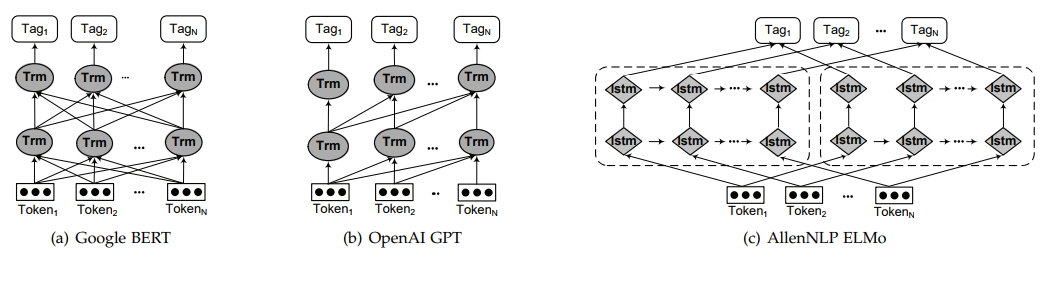
\includegraphics[width = 10cm]{Imagenes/LM.png}
	\caption{Diferencias entre las arquitecturas de los modelos pre-entrenados. \textbf{BERT} usa un Transformer bidireccional (abreviado como \textbf{Tmr}). \textbf{OpenAI GPT} usa un Transformer de izquierda a derecha. \textbf{ELMo} usa la concatenacion de dos LSTM entrenadas independientemente de izquierda a derecha y de derecha a izquierda respectivamente}\label{fig:LM}
\end{figure}

\begin{figure}[h!]
	\centering
	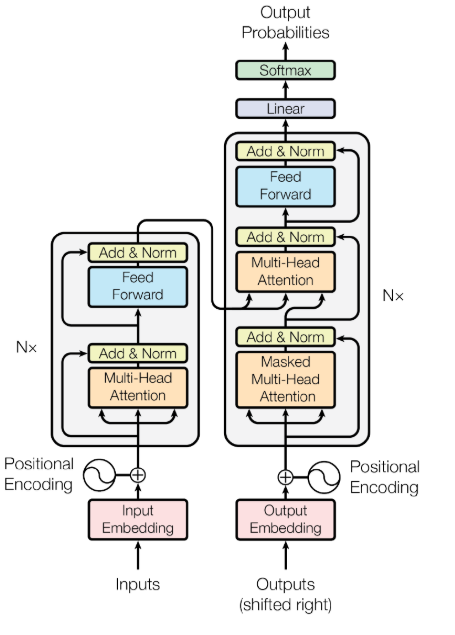
\includegraphics[width = 10cm]{Imagenes/Transformer.png}
	\caption{Arquitectura Transformer.}\label{fig:transformer}
\end{figure}


\subsection{Arquitecturas de Decodificaci\'on de Etiquetas}

La decodificaci\'on de etiquetas es la etapa final en un modelo para NER. Toma como entrada las representaciones dependientes del contexto y produce una secuencia de etiquetas correspondiente a la secuencia de entrada.

Una capa para la decodificaci\'on de etiquetas es la \emph{multi-layer Perceptron + Softmax} donde la tarea del etiquetado de secuencias es tratada como un problema de clasificaci\'on m\'ultiple. La etiqueta para cada palabra es independientemente predicha basado en las representaciones dependientes del contexto sin tener en cuenta sus vecinos. Ejemplo de modelo para NER que usa esta capa para la decodificaci\'on es~\cite{li2017leveraging}.

%Otra capa son los \emph{Conditional Random Fields} (\textbf{CRF}) que es un campo aleatorio globalmente condicionado en las observaciones de la secuencia~\cite{lafferty2001conditional}. Los \textbf{CRF} son un modelo discriminativo que modela los l\'imites de decisi\'on entre las diferentes clases en las que se puede clasificar un elemento de una secuencia.

Otra capa son los \emph{Conditional Random Fields} (\textbf{CRF}) que es un campo aleatorio globalmente condicionado en las observaciones de la secuencia~\cite{lafferty2001conditional}. Los CRF han sido usado ampliamente en aprendizaje supervisado basado en rasgos. Muchos modelos de NER utilizan CRF como su decodificador de etiquetas, como ejemplo de un CRF encima de una capa LSTM es~\cite{peters2018deep} y encima de una CNN es~\cite{collobert2011natural}. Sin embargo, CRF no puede hacer un uso completo de la informaci\'on a nivel de segmentos porque las propiedades internas de los segmentos no pueden ser completamente codificadas con representaciones a nivel de palabra~\cite{li2018survey}. \emph{Zhuo et al.}~\cite{zhuo2016segment} propuso el \emph{gated recursive semi-markov CRF}, el cual directamente modela los segmentos en vez de palabras y automaticamente extrae rasgos a nivel de segmentos a trav\'es de una \emph{gated recursive convolutional neural network}. Recientemente \emph{Ye and Ling}~\cite{ye2018hybrid} propusieron un h\'ibrido \emph{semi-Markov CRF} para el etiquetado de secuencias a partir de redes neuronales. Este acercamiento adopta segmentos en vez de palabras como su unidad b\'asica para la extracci\'on de rasgos y modelado de transiciones. Las etiquetas a nivel de palabras son utilizadas para derivar puntuaciones de segmentos. As\'i que este acercamiento es capaz de subir el nivel tanto de la informaci\'on a nivel de palabra como a nivel de segmento para cada c\'alculo de la puntuaci\'on de un segmento.

Algunos estudios como~\cite{zheng2017joint},~\cite{vaswani2016supertagging} han explorado RNN para la decodificaci\'on de etiquetas. \emph{Shen et al.}~\cite{shen2017deep} report\'o que las RNN superan a los CRF y son m\'as r\'apidas de entrenar cuando el n\'umero de tipos de entidades es grande.

%\emph{Pointer Networks} utilizan \textbf{RNNs} para aprender la probabilidad condicional de una secuencia de salida con elementos que son \emph{tokens} discretos correspondientes a las posiciones en la secuencia de entrada~\cite{vinyals2015pointer}. Representan diccionarios de tama\~nos variables usando la distribuci\'on de probabilidad \emph{softmax} como un puntero. \emph{Zhai et al.}~\cite{zhai2017neural} aplic\'o por primera vez \emph{Pointer Networks} para producir secuencia de etiquetas.

En la figura~\ref{fig:tagDec} se aprecia las diferencias entre algunos de los decodificadores de etiquetas antes presentados.

\begin{figure}[h!]
	\centering
	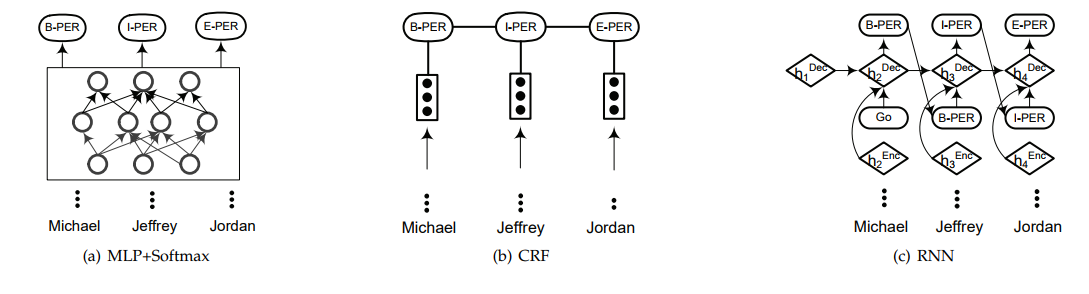
\includegraphics[width = 10cm]{Imagenes/TagDecoders.png}
	\caption{Diferencias entre 3 decodificadores de etiquetas: \textbf{MLP + Softmax}, \textbf{CRF}, \textbf{RNN}.}\label{fig:tagDec}
\end{figure}


\subsection{T\'ecnicas de Deep Learning para NER}
En las \'ultimas secciones se ha hecho un resumen de las t\'ipicas arquitecturas para enfrentar el problema de NER. En esta secci\'on presentamos t\'ecnicas de \emph{Deep Learning} recientemente aplicadas a NER.

\begin{description}
	\item[Deep Multi-Task Learning] Trabajos como~\cite{collobert2011natural} han entrenado modelos para conjuntamente enfrentar las tareas de \textbf{POS}, \textbf{Chunk}, \textbf{NER} y \textbf{SRL}. El trabajo de \emph{Yang et al.}~\cite{yang2016multi} propuso un modelo conjunto \emph{multi-task}, para aprender regularidades espec\'ificas del lenguaje, entrenando conjuntamente en las tareas de POS, NER, Chunk. La idea del \emph{multi-task learning} ha sido aplicada adem\'as para entrenar modelos conjuntos para NER y a su vez la extracci\'on y clasificaci\'on de relaciones~\cite{zhou2017joint} o adem\'as modelar NER como dos subtareas relacionadas, la segmentaci\'on de entidades y la predicci\'on de las categor\'ias de las entidades~\cite{aguilar2019multi}. En el dominio biom\'edico, debido a las diferencias en los distintos conjuntos de datos, la tarea de NER en cada conjunto de datos es considerada una tarea en una configuraci\'on \emph{multi-task}~\cite{wang2019cross}. La principal suposici\'on es que los diferentes conjuntos de datos comparten la misma informaci\'on a nivel de caracteres y de palabras, entonces \emph{multi-taks learning} es aplicado para hacer un uso m\'as eficiente de los datos y alentar al modelo a aprender representaciones m\'as generalizadas.
	
	\item[Deep Transfer Learning] En NLP, \emph{trasnfer learning} es tambi\'en conocido como adaptaci\'on de dominio. En las tareas de NER el acercamiento tradicional para aplicar trasnfer learning es a trav\'es de los algoritmos de \emph{bootstrapping}~\cite{wu2009domain}. Recientemente, nuevos acercamientos como~\cite{lee2017transfer} y~\cite{giorgi2018transfer}  han propuesto usar redes neuronales profundas para la adaptaci\'on de dominio en NER.
	
	\item[Deep Active Learning] Precisamente porque el reentrenamiento desde el inicio no es pr\'actico para aprendizaje profundo \emph{Shen et al.}~\cite{shen2017deep} propuso un entrenamiento incremental para NER con cada \emph{batch} de nuevas etiquetas. La idea, es mezclar nuevos ejemplos anotados con algunos ya existentes, y actualizar los pesos de la red neuronal para un n\'umero peque\~no de \emph{epochs}, antes de consultar por etiquetas en una nueva ronda. Espec\'ificamente, al inicio de cada ronda, el algoritmo de \emph{active learning} elige oraciones para ser anotadas, que pertenecen a un grupo de oraciones predefinido. Los par\'ametros del modelo son actualizados por el entrenamiento en el conjunto de datos aumentado, despu\'es de recibir las anotaciones seleccionadas.
	
	\item[Deep Reinforcement Learning] \emph{Narasimhan et al.}~\cite{narasimhan2016improving} model\'o la tarea de extracci\'on de informaci\'on como un proceso de decisi\'on de \emph{Markov} (\textbf{MDP}), el cual din\'amicamente incorpora predicci\'on de entidades y provee de flexibilidad para elegir las siguiente consulta de b\'usqueda en un conjunto de alternativas autom\'aticamente generado.
	
	\item[Deep Adversarial Learning] \emph{Dual adversarial transfer network} (\textbf{DATNet}), propuesto en~\cite{zhou2018datnet} apunta a lidiar con el problema de los bajos recursos en NER. Los autores preparan una muestra adversarial a\~nadiendole a la muestra original una perturbaci\'on acotada por una peque\~na norma $\epsilon$ para maximizar la funci\'on de p\'erdida como sigue:
	
	\begin{equation}
	\eta_x = arg \ max_{\eta:\lVert \eta \rVert_2 \ \leq \ 2 } \ l(\theta; x + \eta)
	\end{equation}
	
	donde $\theta$ es el conjunto actual de par\'ametros del modelo, $\epsilon$ puede ser determinado en el conjunto de validaci\'on. Un ejemplo adversarial es construido por $x_{adv} = x + \eta_x$. El clasificador es entrenado en la mezcla de los ejemplos originales y los adversariales para mejorar la generalizaci\'on.
	
	\item[Neural Attention] Aplicando mecanismos de atenci\'on, un modelo de NER puede capturar los elementos m\'as informativos de las entradas. Existen muchas formas de aplicar el mec\'anismo de atenci\'on en las tareas de NER. \emph{Rei et al.}~\cite{rei2016attending}, aplic\'o el mecanismo de atenci\'on para din\'amicamente decidir cu\'anta informaci\'on utilizar de una componente a nivel de caracteres o palabras en un modelo de NER \emph{end-to-end}. \emph{Zukov-Gregoric et al.}~\cite{zukov2017neural} explor\'o el mecanismo de \emph{self-attention} en NER, donde los pesos son dependientes de una sola secuencia.
\end{description}


%\subsubsection{Deep Multi-Task Learning}

%\emph{Multi-task learning} es un acercamiento que aprende un conjunto de tareas juntas~\cite{caruana1997multitask}. Si se consideran las relaciones entre las diferentes tareas, se espera que los algoritmos de \emph{multi-task learning} consigan mejores resultados que aquellos que aprenden una tarea individualmente~\cite{li2018survey}.




%\subsubsection{Deep Transfer Learning}
%
%\emph{Transfer Learning} apunta a lograr un mejor desempe\~no de una tarea de aprendizaje de m\'aquina en un dominio espec\'ifico tomando ventaja del conocimiento aprendido del dominio fuente~\cite{pan2009survey}. En \textbf{NLP}, \emph{trasnfer learning} es tambi\'en conocido como adaptaci\'on de dominio. 

%En las configuraciones de \emph{transfer learning} diferentres modelos neuronales comunmente comparten diferentes partes de los par\'ametros del modelo entre la tarea fuente y la tarea objetivo. \emph{Yang et al.}~\cite{yang2017transfer} fue el primero en investigar la transferibilidad de las diferentes capas de representaci\'on, entonces presentaron 3 diferentes arquitecturas para compartir par\'ametros entre escenarios de \emph{cross-domain}, \emph{cross-lingual} y  \emph{cross-application}. En particular si dos tareas tienen conjuntos de etiquetas mapeables, entonces hay una capa de \textbf{CRF} compartida, en otro caso cada tarea tiene su propia capa de \textbf{CRF}. Otros trabajos de \emph{trasnfer learning} en \textbf{NER} son~\cite{von2017transfer},~\cite{zhao2018improve},~\cite{lin2018neural},~\cite{giorgi2018transfer}.

%\subsubsection{Deep Active Learning}

%La idea esencia detr\'as de \emph{deep active learning} es que un algoritmo de aprendizaje de m\'aquina pueda desempe\~narse mejor con una cantidad substancial menor de datos de entrenamiento, si se permite elegir los datos con los que entrenar\'a~\cite{settles2012active}. Aprendizaje profundo requiere una gran cantidad de datos de entrenamiento que es costoso de obtener. Por lo tanto, combinando aprendizaje profundo con \emph{active learning} se espera que se reduzca el esfuerzo de anotaci\'on de los datos.

%Entrenamiento con \emph{active learning} procede en m\'ultiples rondas. Sin embargo, los esquemas tradicionales de \emph{active learning} son costosos para aprendizaje profundo, porque despu\'es de cada ronda requiere un reentrenamiento completo del clasificador con nuevos datos anotados. 

%\subsubsection{Deep Reinforcement Learning}

%\emph{Reinforcement Learning} es una rama del aprendizaje de m\'aquinas inspirada por la psicolog\'ia del comportamiento, que tiene que ver con c\'omo agentes de software toman acci\'on en el ambiente con el objetivo de maximizar alguna recompensa acumulativa~\cite{kaelbling1996reinforcement},~\cite{sutton1998introduction}. La idea es que el agente aprender\'a a partir de la interacci\'on con el ambiente y recibiendo recompensas por realizar acciones. Especifiamente el problema del \emph{reinforcement learning} puede ser formulado de la siguiente forma~\cite{hoi2018online}: el ambiente es modelado como una m\'aquina de estado estoc\'astica finita con entradas (acciones del agente) y salidas (observaciones y recompensa del agente). Esto consiste en 3 componentes claves:
% 
% \begin{enumerate}
% 	\item La funci\'on de transici\'on de estados.
% 	\item La funci\'on de observaciones (o sea, salida).
% 	\item La funci\'on de recompensa.
% \end{enumerate}
% 
%El agente es tambi\'en modelado como una m\'aquina de estado estoc\'astica finita con entradas (observaciones y recompensas del ambiente) y salidas (acciones en el ambiente). Esto consiste en dos componentes: (i) una funci\'on de transici\'on de estado, y (ii) una funci\'on de salida. La meta final del agente es aprender una buena funci\'on de actualizaci\'on de estado intentando maximixar las recompensas acumuladas.



%\subsection{Deep Adversarial Learning}

%\emph{Adversarial Learning} es el proceso de explic\'itamente entrenar un modelo en ejemplos adversariales. El prop\'osito es hacer el modelo m\'as robusto contra ataques o reducir sus test error on clean inputs. \emph{Adversarial networks} aprenden a generar a partir de una distribuci\'on de entrenamiento a trav\'es de un juego de dos jugadores: una red genera candidatos (\emph{generative network}) y la otra los eval\'ua (\emph{discriminative network}). T\'ipicamente, la red generativa aprende a mapear de un espacio latente a una distribuci\'on particular de los datos de inter\'es, mientras que la red discriminativa discrimina entre los candidatos generados por el generador e instancias de la distribuci\'on de datos del mundo real~\cite{goodfellow2014generative}.




%\subsection{Neural Attention}

%El mecanismo de \emph{attention} en una red neuronal es basado en el mecanismo de atenci\'on virtual del humano~\cite{britz2016attention}. El mecanismo de \emph{neural attention} permite a las redes neuronales la habilidad de enfocarse en un subconjunto de sus entradas. 

\section{Extracción de Relaciones}

\section{Enfoque Conjunto}
%===================================================================================

